\documentclass[12pt]{article} 
\usepackage[pdftex]{graphicx}
\usepackage{natbib} 
\usepackage{color}
\usepackage{amsmath} 
\usepackage{amssymb} 
\usepackage{verbatim}
\usepackage{mathpazo} 
\usepackage{setspace}
\usepackage{multirow}
\usepackage{fullpage}
\usepackage{lscape}
\usepackage{fancyhdr}
\usepackage[normalem]{ulem} 
\usepackage{hyperref}
\usepackage[parfill]{parskip}
\usepackage{graphicx}
\usepackage{longtable}
\usepackage{times}
\usepackage{textcomp}
\usepackage{xr}
\usepackage{etoolbox}
\usepackage{filecontents}
\usepackage{url}
\externaldocument{SI}
\hypersetup{colorlinks=true, linkcolor=black, citecolor=black}
\RequirePackage{lineno}

\newcommand{\flagged}[1] {
  \textcolor{blue}{#1}
}

\def\title{The temporal assembly of plant-pollinator networks
  following restoration}
\def\author{Lauren C.\ Ponisio$^{1,2}$, Marilia P. Gaiarsa$^3$, Claire
  Kremen$^1$}

\def\runninghead{Plant-pollinator network assembly}
\def\keywords{community assembly, change points, specialization,
  nestedness, modularity, bipartite, preferential attachment}

\def\extras{
  \begin{itemize}
  \item Submitted as a Letter
  \item Abstract word count: 
  \item Main text word count: 
  \item Number of references: 
  \item Number of figures:
  \end{itemize}
}

\def\affiliation{
  \begin{enumerate}
  \item Department of Environmental Science, Policy, and Management\\
    University of California, Berkeley\\
    130 Mulford Hall\\
    Berkeley, California, USA\\
    94720\\
  \item Department of Entomology\\
    University of California, Riverside\\
    417 Entomology Bldg.\\
    Riverside, California, USA\\
    92521\\
  \item Departamento de Ecologia\\
    Universidade de Sao Paulo\\
    Sao Paulo, SP, Brazil\\
    05508-900\\
  \end{enumerate}
}

\newcommand{\mstitlepage}{
  \paragraph{Running head:} \textsc{\runninghead}
  % \parindent=0pt
  \begin{center}%
    {\LARGE \title \par}%
    \vskip 3em%
    {\large
      \lineskip .75em%
      \begin{tabular}[t]{c}%
        \author
      \end{tabular}\par}%
    \vskip 1.5em%
  \end{center}\par
  \affiliation
}
\clearpage

\begin{document}

\mstitlepage
\doublespacing
\linenumbers
\clearpage

\begin{abstract}
  TO BE RE-WRITTEN
  The structure of networks is related to ability of communities to
  maintain function in the face of species extinction. Understanding
  network structure and how it relates to network disassembly,
  therefore, is a priority for system-level conservation biology.  We
  explore the assembly of plant-pollinator communities on native plant
  restorations in the Central Valley of California. 
\end{abstract}

Keywords: changing points, temporal networks, hedgerows, species
interactions, preferential attachment, mutualisms

\clearpage

\section*{Introduction}
\label{sec:introduction}

%% introduce mutualisms, restoration, network assembly
Global change has created a severe biodiversity crisis, and as species
are lost, so are their interactions \citep{dunn2009sixth,
  barnosky2011has}. Because mutualistic interactions are essential for
maintaining the diversity their component guilds of species, these
systems are particularly at risk from coextinction cascades. The
nature of these coextinction cascades depends on the interaction
patterns within a community \citep{Memmott2004, Rezende2007,
  Bascompte2009}. Recovering the lost biodiversity and interactions
through ecological restoration has become increasingly imperative, and
a key restoration aim is to facilitate assembly of robust interaction
networks \citep{menz-2010-4}. We know little, however, about how to
re-assemble interacting communities through restoration, or the
process of ecological network assembly more generally.

%% most people think network assemble via preferential attachment, and
%% there is some evidence of that. (other studies on mutualisms?)
The mostly widely explored mechanism of network assembly, preferential
attachment \citep{barabasi1999emergence}, predicts that a new species
is more likely to interact with species that are already
well-connected \citep[''the rich-get-richer''
principle,][]{barabasi1999emergence}. In pollination systems --- a
particularly ubiquitous mutualism \citep{ollerton-2011-321,
  klein-2007-303} --- some studies have found support for this
mechanism of assembly. Investigating the day-to-day, temporal assembly
of a plant-pollinator network within a season, \cite{Olesen2008} found
that new species tended to interact with already well-connected
species, likely because these species are either more abundant or more
temporally persistent \citep{Olesen2008}. In addition, using a
space-for-time substitution to study primary succession along a
glacier foreland, \cite{albrecht2010plant} found some indication
assembly was occurring through preferential attachment. Network
nestedness, a pattern of interactions where a generalist core
interacts with both specialist and generalist species, increased as
the community aged \citep{albrecht2010plant}. Increasing nestedness
could result from a process like preferential attachment where
specialist species attach to the well-connected, generalist core.  In
addition, non-successional temporal dynamics also suggest a stable
core of generalists persists despite high turnover of peripheral
species \citep{fang2012relative, diaz2010changes, alarcon2008year}.

%% there are other ways to assemble that are not preferentia;
%% attchment, particularly vis big reorganizations of interactions
In contrast to the ordered network build-up described by preferential
attachment, assembly can be punctuated by significant reorganizations
of interactions \citep{peel2014detecting}. Such significant
reorganizations of interactions, or changing points, have been
observed in social networks responding to abrupt shifts in the
behavior of interactors \citep{peel2014detecting}.  In ecological
communities, such shifts my occur if, as new species are added,
resident species change their interaction partners to optimize their
foraging effort. In plant-pollinator communities, theory predicts
pollinators optimize their use of floral resources to reduce
interspecific competition and improve resource-use efficiency
\citep{pyke1984optimal, valdovinos2010consequences,
  valdovinos2013adaptive, albrecht2010plant, Bluthgen2007}. No
studies, however, have examined whether changing points occur during
ecological network assembly and how they relate to the behavior of the
interactors.

%% restoration
Understanding network assembly is particularly relevant to ecological
restoration, which is essentially 'applied succession'
\citep[e.g.,]{parker1997scale}. In pollination systems, the time since
an area was restored has been shown to effect the structure of
networks \citep{forup-2008-742, forup2008restoration,
  devoto2012understanding}, suggesting interactions are evolving as the
community develops. Understanding the mechanisms of network assembly
will help to guide the restoration of particular communities.

%% restoration of ecosystem services is really important, particularly
%% in ag. but ag is a bad place for pollinators
Facilitating effective restoration of networks is especially
imperative in areas where species interactions provide essential
ecosystem services, such as crop pollination. In intensively managed
agricultural landscapes, the demand for pollination services is the
greatest \citep{kremen-2008-10}. However, honey bees, managed
extensively around the world to provide crop pollination, are in
global decline \citep{neumann-2010-1, van-engelsdorp-2009-e6481}. In
addition, native pollinators, which have the capacity to provide
sufficient crop pollination \citep{kremen-2002-16816,
  winfree-2007-1105, kremen-2004-1109}, are in short supply because
these landscapes make poor habitats for pollinator populations
\citep{kremen-2002-16816}. To ensure provision the continued provision
of ecosystem services and curb biodiversity loss, effective
restoration of pollinators and their interactions in agricultural
landscapes is critical.

%% hedgerows!!  
To promote pollinator services in agriculture, farmers are
increasingly turning to the habitat restoration technique of planting
strips of native plants along farm edges (hedgerows) to help provide
habitat for pollinators without removing arable land from
production. Hedgerows have been shown to augment the richness,
abundance and trait diversity of pollinators in agricultural
landscapes\citep{morandin-2013-829, mgonigle-2015-x, kremen-2015-602,
  ponisio2015farm}. In addition, hedgerows promote the persistence and
colonization of floral resource specialists
\citep{mgonigle-2015-x}. Little is known however, about the assembly
of the network following hedgerow restoration. 

Using a long-term data-set of plant-pollinator communities assembling
following hedgerow restoration in the highly simplified and
intensively managed agricultural landscape of California's Central
Valley, we explore the process of network development. We first
determine whether the mechanism underlying network assembly is a
smooth build up of interactions as would be predicted by preferential
attachment, or punctuated by significant reorganizations of
interactions (i.e., changing points). Even with changing points in
interaction organization, networks could still be assembling via
preferential attachment if the network reorganizations were primarily
driven the by peripheral, temporally variable species while a stable,
well-connected core of species still persists. We thus examine whether
the species are most variable in their network position --- and thus
important contributors network reorganizations --- are less persistent
and connected species.  Lastly, we examine whether networks are
assembling toward predictable interaction patterns, and the
ramifications for the robustness of the networks to species extinction
and cascading perturbations.

%% objectives
% 1) Are hedgerows assembling by preferential attachment, or are there
% more abrupt reorganizations of network structure?
% 2) Who are the species responsible for interaction reorganizations?
% how to incorporate this? 
% 3) Are the changing points a product of turnover in species
% composition, or are more substantial changes in the verticles of the
% networks?
% 4) Is the structure of interactions changing? Does this change the
% robustness of the network to species extinction and/or perturbation?

\section*{Materials \& Methods}
\label{sec:methods}

\subsection*{Study sites and collection methods}
\label{sec:study-sites}

We surveyed plant-pollinator interaction networks of assembling
hedgerows (N=5), as well as in two types of non-assembling communities
to serve as controls: unrestored, weedy field margins (N=19) and
established hedgerows (greater than 10 years since planting,
N=29). The sites were located in the Central Valley of California in
Yolo, Colusa and Solano Counties. This area is comprised of
intensively managed agriculture -- primarily monocultures of
conventional row crops, vineyards and orchards. Hedgerows we planted
along field margins where they do not remove valuable land from
production, and are ca. 3--6m wide and approximately 350m long and
border large (ca.\ 30--hectare) crop fields. Hedgerows consist of
native, perennial, shrub and tree plantings including \textit{Rosa
  californica}, \textit{Cercis occidentalis}, \textit{Ceanothus spp.},
\textit{Heteromeles arbutifolia}, \textit{Sambucus mexicana},
\textit{Eriogonum spp.}, \textit{Baccharis spp.}, \textit{Salvia
  spp}. and others \citep{kremen-2015-602, mgonigle-2015-x}. The mean
distance between monitoring sites was 15 km, and the minimum distance
between sites of the same type sampled in the same year was 2 km.  The
entire area surveyed spanned almost 300 km$^2$. The crop fields
adjacent to all sites were similarly managed as intensive, high-input
monoculture.

Monitoring began in 2006 and continued through 2015. Sampling of the
assembling hedgerows began the year before the area was restored. For
logistical reasons, no sampling of assembling hedgerows was conducted
in 2010. Sites were sampled between two and five times per year
(Tables S1-S3). In each round of
sampling, the order in which sites were sampled was
randomized. Surveys were conducted under sunny conditions when the
temperature was above $21^{\circ}\mathrm{C}$ and wind speed was below
$2.5$ meters/second.

Flower-visitors to plants in hedgerows and unrestored controls were
netted for one hour of active search time (the timer was paused when
handling specimens). Honeybees (\textit{Apis mellifera}) were not
collected because their abundance is determined largely by the
placement of hives throughout the region by bee-keepers. All other
insect flower visitors that touched the reproductive parts of the
flower were collected; however, here we focus only on wild bees and
syrphids (representing 49 and 19 percent of records, respectively),
the most abundant and effective pollinators in the system (C. Kremen,
A.~Klein and L.~Morandin, unpublished data). Bee and syrphid specimens
were identified to species (or morpho-species for some bee specimens
in the genera \textit{Nomada} and \textit{Sphecodes}) by expert
taxonomists.

Quantitative networks were generative for each site through time. To
account for the unequal number of surveys between years, the mean of
the interactions between a pair of plants and pollinators across
surveys within a year was used as a representation of the frequency of
interactions.

\subsection*{Change point analysis}
\subsubsection*{Identifying change points}
We employed a change point detection method \citep{peel2014detecting}
to identify fundamental changes in large-scale pattern of interactions
of plants and pollinators. A change point is caused by a merge, split,
fragmentation or formation of communities (also called modules or
compartments). Change point detection methods have yet to be
generalized to quantitative networks, so for this analysis we focused
on qualitative (binary) networks. Following \cite{peel2014detecting},
we first defined a probability distribution over the networks using
the generalized hierarchical random graph model (GHRG). The GHRG model
is able to capture both assortative and disassortative community
structure patterns at all scales in the network
\citep{peel2014detecting}. A network $G$ is composed of vertices $V$
and edges $E \subseteq {V × V }$. The GHRG model decomposes the $N$
vertices into a series of nested groups, the relationships among which
are represented by the dendrogram $T$. The tips of $T$ are the
vertices of $G$, and the probability that two vertices $u$ and $v$
connect is given by the parameter $p_r$. The probability distribution
of the network $G$ thus defined as:

\begin{equation}
  \label{eq:lik}
  P(G|T,{pr}) = p_r^{E_r}(1-p_r)^{N_r-E_r}
\end{equation}
% 
Where $E_r$ is the observed number of edges between vertices with the
common ancestor $r$, and $N_r$ is the total possible edges.

Using Bayesian posterior inference and techniques from phylogenetic
tree reconstruction, we fit the GHRG model to the networks
\citep{peel2014detecting}. This is accomplished by using a Markov
Chain Monte Carlo (MCMC) procedure to first sample the posterior
distribution of bipartitions, from which a consensus tree is derived
\citep{peel2014detecting}. We used $\beta$ distributions with the
hyperparameters $\alpha=\beta=1$ to define priors for $p_r$.

Once the GHRG model has been fit to the networks, we determine whether
a change point occurred between two time slices. To detect a change
point, we compare the fit of two models -- one where a change point
had occurred between two networks, and one where no change occurred --
using posterior Bayes factors. We chose a sliding window of length,
$w$, of four, within which to find change points. Larger windows allow
for more gradual changes, and four was the maximum possible with our
maximum of nine years of data. Lastly, to calculate a $p$-value for
the Bayes factors, we use parametric bootstrapping to numerically
estimate the null distribution \citep{peel2014detecting}. The change
point analysis was carried out using code published online by
L.~Peel. Analyses we conducted in Python 3.4.

We next test whether the change points occurring in maturing hedgerows
were a component of the assembly process or a product of environmental
shifts that lead to network reorganizations in all types of
communities. We model the number of change points as successes and the
total number of years each site was sampled as trails, and use a
generalized linear model with Binomial error to test whether the
probability of a change point occurring varied by site type. For the
non-assembling hedgerows and weedy field margins, only sites with five
or greater years of sampling was included in this analysis. All
statistical analysis were conducted in R 3.2.3 \citep{R}.

\subsubsection*{Characteristics of species that contribute to change
  points}

To further elucidate the nature of the change points, we examine the
characteristics of the species that contributed the reorganization of
interactions. Some species remain in relatively similar network
positions through time, whereas others are more variable in their role
and thus contribute more strongly to network reorganization. We test
the that more persistent species with the highest degree are the most
stable in their network position, as would be expected is the networks
were assembling via preferential attachment.

We calculate species persistence as the proportion of the surveys a
pollinator was observed. Species observed consistently within and
between years are thus maximally persistent. Weighted species degree
is calculated from interaction observations observed in more extensive
data-set from Yolo County (approx.~18000 interaction records) that
included both the data included in this study and additional data from
sites where we collected flower visitors using the same methods
\citep{mgonigle-2015-x, ponisio2015farm}. %% does this make sense to
%% calculate from an independent data set?
To represent the the variability of species within networks, we
computed the coefficient of variation of weighted closeness at each
site through time. Closeness describes the centrality of a species in
the network by calculating path lengths to other vertices (species) in
the graph. We used linear mixed models to test whether the variability
of species closeness values was related to the persistence or degree
of that species \citep{lme4, lmetest}. We included random effects for
species, as well as site. We focused on the pollinator species because
the hedgerow flowers are planted and thus are not directly
assembling. Because degree and persistence were strongly correlated,
($\rho = 0.84$, $p$-value $<$ $2*10^{-16}$), each explanatory variable
was included in the model separately. Because a linear increase in
closeness, as might be expected with assembly by preferential
attachment, would lead to a high variability in closeness scores, we
also test whether closeness increases through time.

\section*{Temporal changes in interaction patterns}
\subsection*{Network structure}
Any changing points in network structure may contribute to the
reorganization of the assembling networks into predictable interaction
patterns. Pollination networks exhibit two main structural patterns
--- modularity \citep[e.g.,][]{Olesen2007} and nestedness
\citep[e.g.,][]{Bascompte2006, Bascompte2003}. In modular networks,
interactions are insular, occurring within separate groups or
``modules'' more often than between modules. Communities in the
network may fragment as the network assembles, enhancing
modularity. Conversely, nested networks are like pyramid of
interactions, where there are some species that interact with many
species, other species that interact with a subset of those species,
and so on. If species entering the network tend to interact with the
generalist base of the network pyramid (i.e., via preferential
attachment), nestedness would increase through time. Lastly, if the
network is accumulating specialist species or species are beginning to
limit their interaction niche breath as the network assembles, this
would lead to an increase in the network-level specialization
\citep{bluthgen-2006-9}. To test whether network modularity,
nestedness or specialization changed linearly with assembly, we used
linear mixed models with the descriptive network metrics as the
response variable, year of assembly as the explanatory variable, and
random effects of site and year.

We use NODF (weighted or unweighted) to evaluate network nestedness
\citep{nodf}. NODF evaluates whether species with fewer partners
interact with subsets of partners with which more connected species
interact \citep{nodf}. To estimate modularity, we use a hierarchical
clustering algorithm \citep{Newman2004, igraph}.  We calculated
standardized $z$-scores so that nestedness and modularity metrics
could be compared between communities. The $z$-scores were calculated
by generating an ensemble of $999$ randomly assembled communities,
subtracting the mean of the statistic calculated across these
communities from the observed value, and then dividing by the standard
deviation. To assemble random communities, we reshuffled the
interactions between species but fixed the total number of
interactions, species and the distribution of the interaction
frequencies \citep{Galeano2009}. Lastly, Network specialization was
measured using H2, which estimate the deviation of the observed
interaction frequency between plants and pollinators from a null
expectation where all partners interact in proportion to their
abundances \citep{bluthgen-2006-9}. It ranges from 0 for generalized
networks to 1 for specialized networks.


\subsection*{Network robustness}
Lastly, we test the changes in interaction patterns associated with
network assembly affect the robustness of the network to species loss
and to cascading perturbations. Following \cite{Memmott2004}, we simulate
the extinction of plant species the subsequent extinction cascades of
pollinator species. Because the reproduction of plant species if
facilitated by active restoration efforts, it is unlikely the
extinction of pollinators would affect plant populations in the
hedgerows. However, plants ceasing to bloom, for example in response
to drought, will likely affect the pollinators that depend on
them. Plants species were eliminated based on their degree or
abundance, and the number of pollinators that secondarily went extinct
is calculated. The area below the extinction curve is used as a
measure of network robustness \citep{bipartite}.

We also explored how the robustness to cascading perturbations changed as
community assembled, using algebraic connectivity --- the second
smallest eigenvalue of the Laplacian matrix
\citep{fiedler1973algebraic} --- as a proxy for network robustness
(Gaiarsa et al., submitted). Algebraic connectivity is related to how difficult it is to turn a network
into completely disconnected groups of nodes, or species
\citep{costa2007characterization} --- the larger the algebraic
connectivity, the more robust a network is to cascading perturbations
(Gaiarsa et al., submitted), and the harder it is to break the
community into isolated groups of species.



\section*{Results}
\label{sec:results}

Over eight years and $747$ samples, we collected and identified
$19,547$ wild bees and syrphids comprising $173$ species from $50$
genera. We observed $1,521$ unique interactions between plants and
pollinators.

\subsection*{Change point analysis}
\subsubsection*{Identifying change points}

The majority ($76\%$) of the sites tests underwent at least one
significant reorganization of interactions
(Fig.~\ref{fig:changePoints}).  All five of the assembling hedgerows
experienced changing points, whereas only $40\%$ and $81\%$ of
non-assembling hedgerows and field margins, respectively, underwent
significant interaction reorganizations. Assembling hedgerows
experienced significantly more changing points than the non-assembling
networks (difference in the odds ratios between assembling and
non-assembling networks, $3.316$, $95\%$ CI $[1.314, 8.572]$,
$p$-value= $0.0117$). Network assembly following restoration is thus
punctuated by more interaction reorganizations than would be expected
by environmental shifts that would effect assembling and
non-assembling networks equally.

\begin{figure}
  \centering
  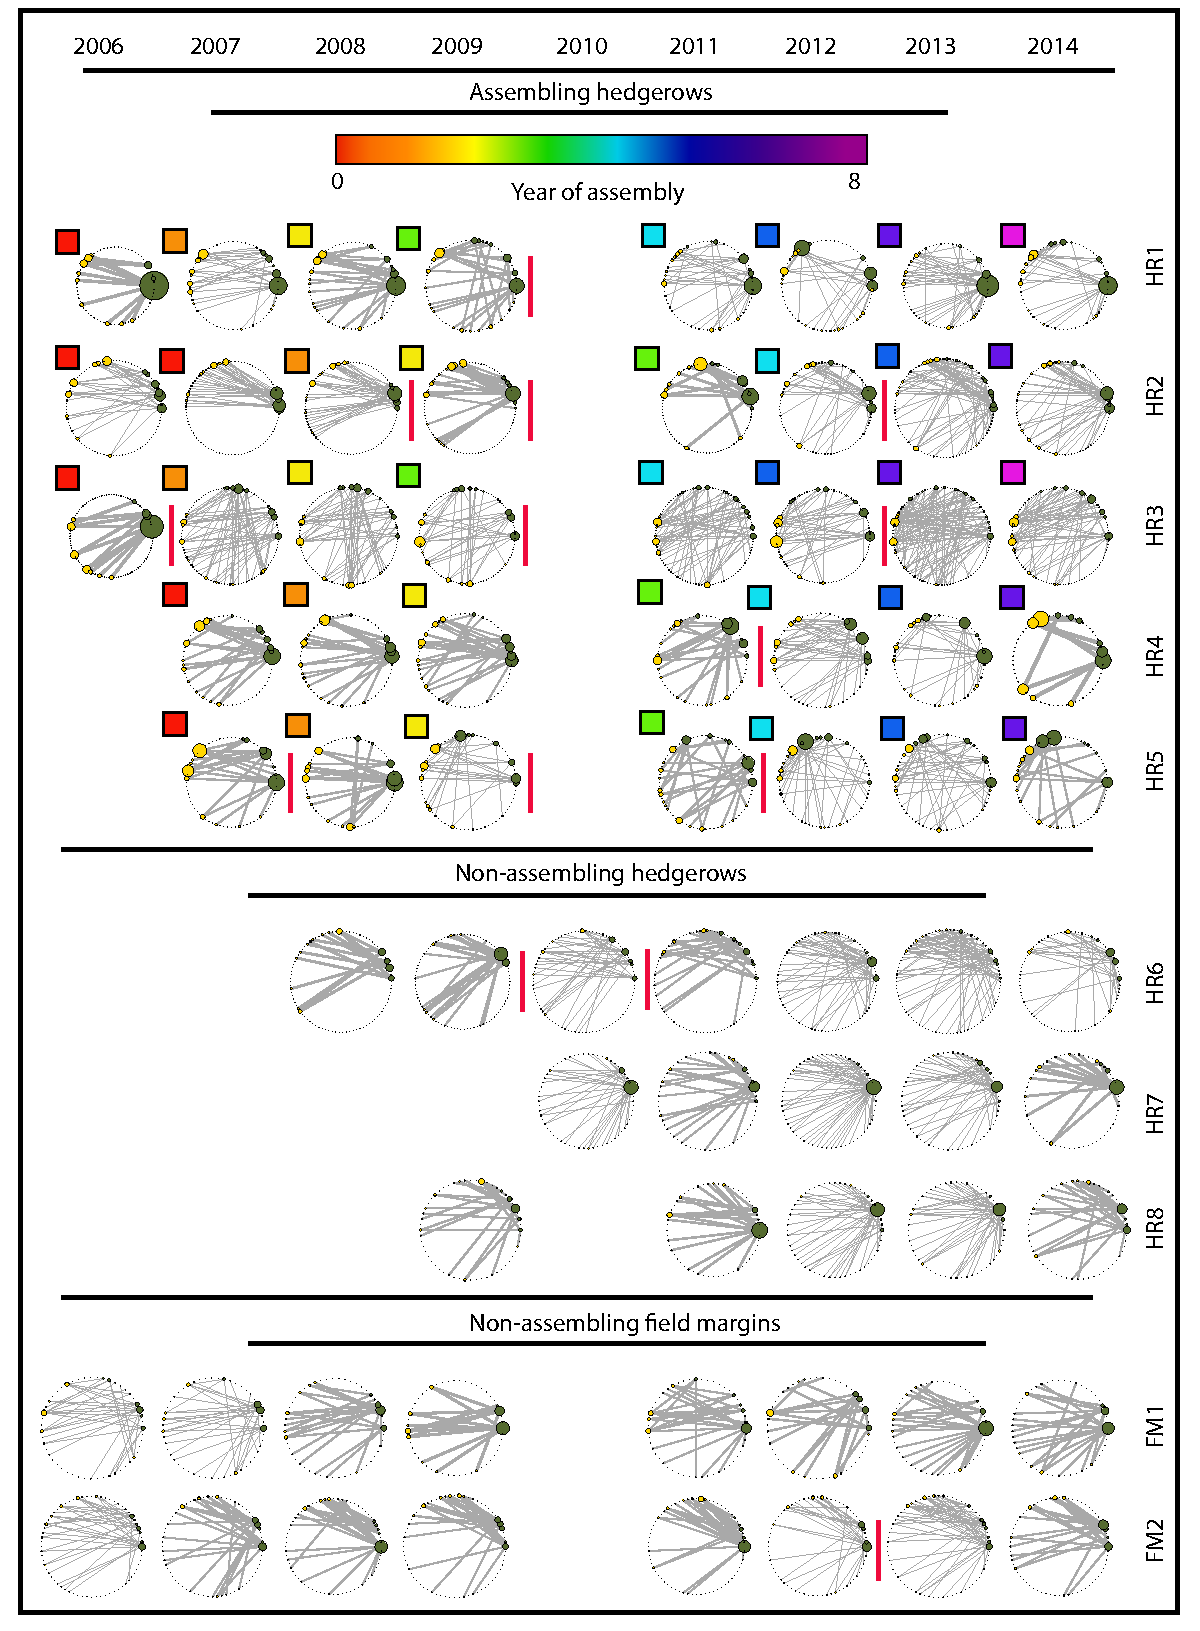
\includegraphics[width=.8\textwidth]{../analysis/changePoint/plotting/networks.pdf}
  \caption{The network structure and changing points (vertical red
    lines) in assembling hedgerows and a representative sample of
    non-assembling hedgerows and weedy field margins. In each network,
    plants and pollinators are represented by green and yellow
    circles, respectively, weighted by their degree. Each species has
    has a consistent position in the network across years. In the
    assembling hedgerows, colored squares in the corner of each
    network represent the years post restoration.}
  \label{fig:changePoints}
\end{figure}
\clearpage

\subsubsection*{Characteristics of species that contribute to change
  points}

In contradiction to the predictions of assembly by preferential
attachment, both pollinator persistence and degree were positively
related to network position variability. (ADD STATS IF KEEPING
RESULT).

\begin{figure}
  \centering
  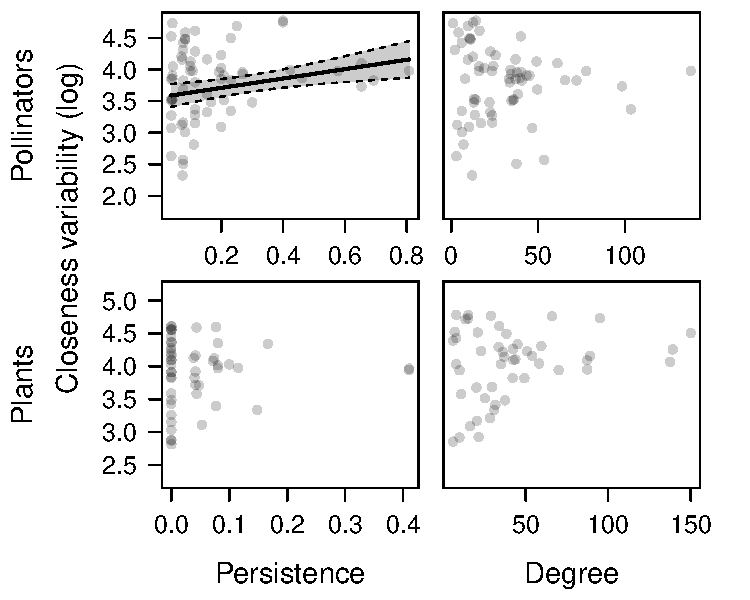
\includegraphics[width=.8\textwidth]{../analysis/variability/figures/cv/occ_degree.pdf}
  \caption{The coefficient of variation of network position, as
    represented by closeness, plotted against pollinator persistence
    and degree. Points represents means for each species across sites.
    The solid line indicates the mean slope estimate and the dashed
    lines are the $95\%$ confidence intervals around the estimate. }
  \label{fig:cv}
\end{figure}
\clearpage

\section*{Temporal changes in interaction patterns}
\subsection*{Network structure}
Network nestedness significantly increased with assembly (estimate of
the slope of nestedness through time $\pm$ standard error of the
estimate, $1.834 \pm 0.6142$, $p$-value=$0.022$, Fig.~
\ref{fig:baci}).  Modularity decreased (Fig.~\ref{fig:baci}), though
the slope was not significantly different from zero (estimate of the
slope of modularity through time $\pm$ standard error of the estimate,
$-0.524$ $\pm$ $0.295$, $p$-value=$0.124$). Specialization remained
relatively constant (estimate of the slope of specialization through time
$\pm$ standard error of the estimate, $0.003$ $\pm$ $0.015$,
$p$-value=$0.827$).


\begin{figure}
  \centering
  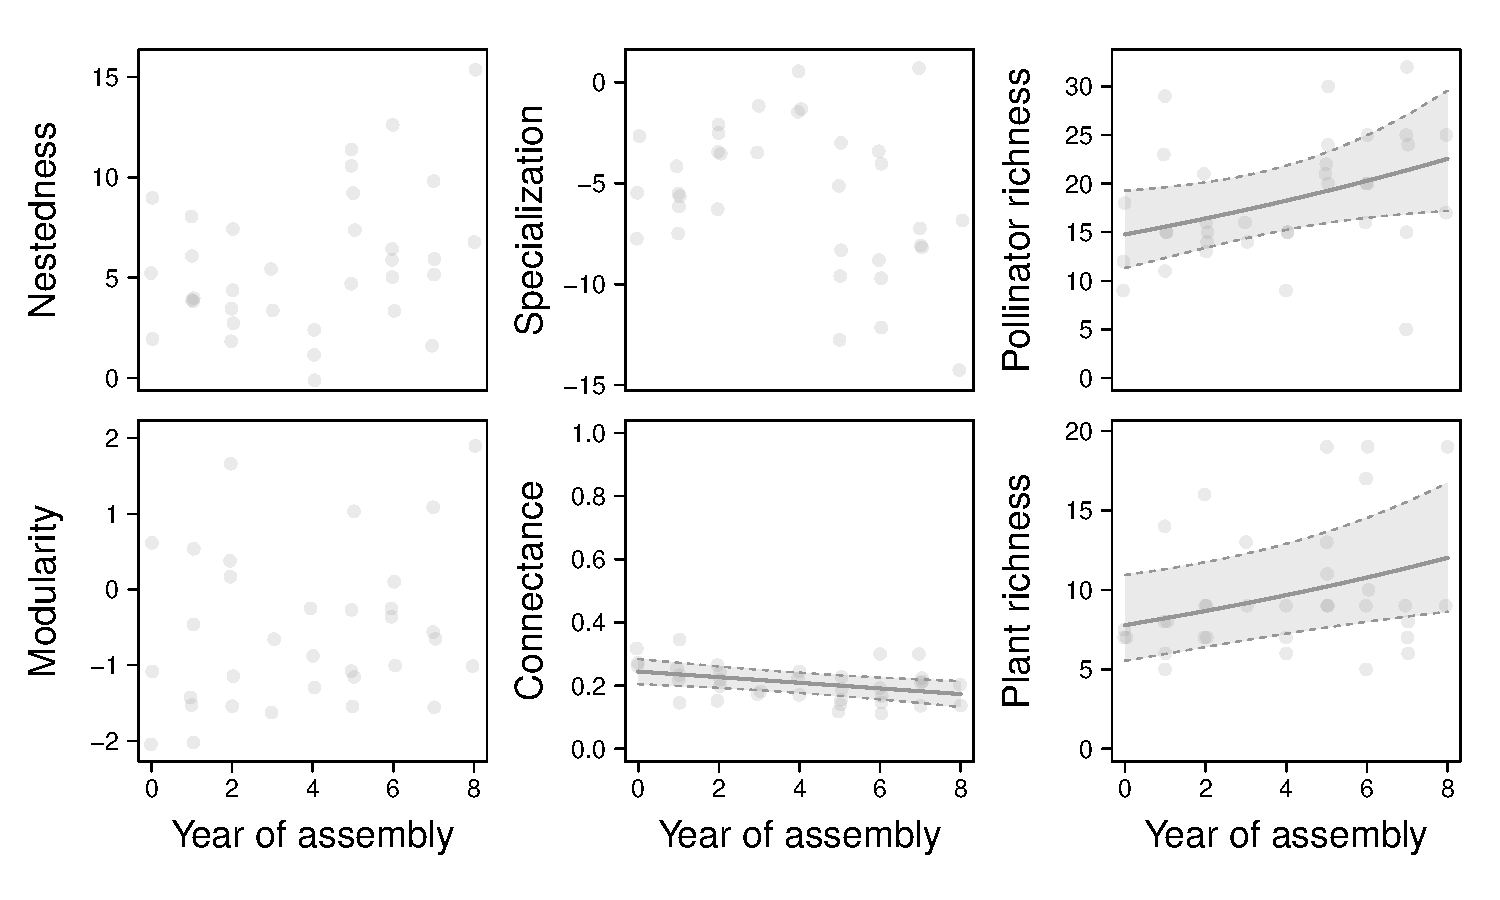
\includegraphics[width=.7\textwidth]{../analysis/networkLevel/figures/baci.pdf}
  \caption{The change in nestedness, modularity, specialization and
    connectance as the networks assemble. The left panels represent
    $z$-scores. Scores greater than $\sim 2$ or less than $\sim -2$
    are significantly more or less structured than randomly assembled
    networks. Points are the value for each site at each year of
    assembly. The solid line indicates the mean slope estimate and the
    dashed lines are the $95\%$ confidence intervals around the
    estimate.}
  \label{fig:baci}
\end{figure}
\clearpage

\subsection*{Network robustness}
Assembly did not effect the robustness of the networks to species
extinction when species where removed incrementally by degree
(estimate of the slope of robustness through time $\pm$ standard error
of the estimate, $6*10^{-5} \pm 4*10^{-3}$, $p$-value=$0.987$) or
abundance ($0.001 \pm 0.003$, $p$-value=$0.65$, Fig.~\ref{fig:rob}).

In contrast, the robustness of networks to cascading perturbations, as
measured by the algebraic connectivity of the network, increased as
the network assembled (estimate of the slope of robustness through
time $\pm$ standard error of the estimate, $0.6814 \pm 0.272$,
$p$-value=$0.042$, Fig.~\ref{fig:rob}).

\begin{figure}
  \centering
  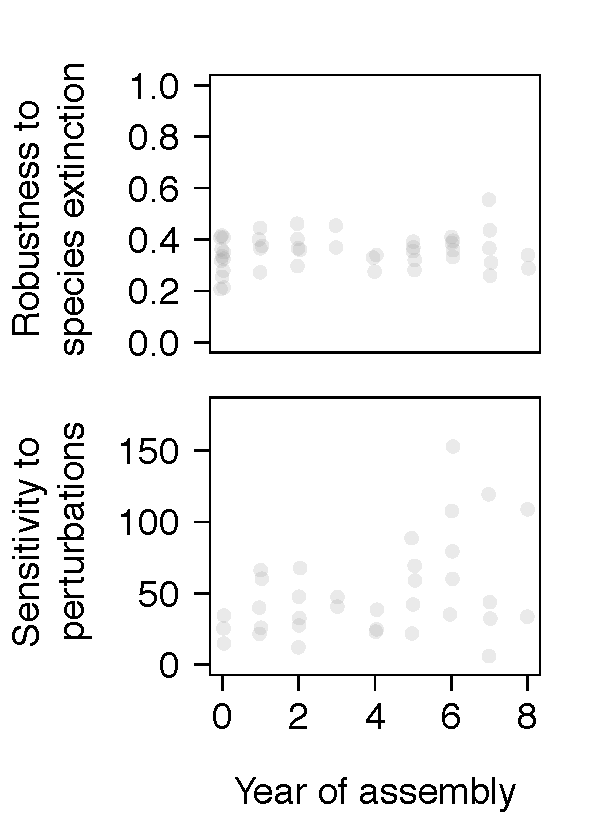
\includegraphics[width=.7\textwidth]{../analysis/networkLevel/figures/robustness.pdf}
  \caption{The robustness of networks to species extinction and
    to cascading perturbations. The robustness to species extinction is measured by
    incrementally removing species by degree, through removing species
    by abundance did not yield qualitatively different results. The robustness of networks to cascading perturbations is measured as the algebraic connectivity, the second smallest eigenvalue of the Laplacian matrix. Points
    are the value for each site at each year of assembly. The solid
    line indicates the mean slope estimate and the dashed lines are
    the $95\%$ confidence intervals around the estimate.}
  \label{fig:rob}
\end{figure}
\clearpage


\section*{Discussion}
\label{sec:discussion}

We show that the temporal assembly of plant-pollinator networks
following restoration is a highly dynamic process where interactions
often undergo significant reorganizations. These network organizations
are unlikely to be a product of environmental forces alone because the
network changing points in non-assembling communities are less
frequent, and there are few consistent trends in when change points
occurred across all sites. Several sites had changing points between
year 2009 and 2011 (Fig.~\ref{fig:changePoints}). In California, 2011
marked the beginning of a multi-year drought. In the assembling
hedgerows were not sampled in 2010, so disentangling whether the
changing points are due to skipping a year of assembly or the drought
is not possible. Interestingly, most of the assembling hedgerows did
not undergo a significant reorganization of interactions immediately
the hedgerow was planted (i.e., the transition from weedy field margin
to hedgerow). This result is consistent with the finding that in our
study system, hedgerow restoration takes several years to have a
significant impact on the plant-pollintor communities (Kremen and
M'Gonigle, in prep).

%% marilia: I see where you are going witht he bluthgen reference, but
%% that seemed like something that should be in the intro or
%% methods. Otherwise it is beinging up a new concept we did not
%% previously explain. 

Given that several changing points in network organization occured
during assembly, we next explored the species most likely responsible
for the shifts in interaciton patterns. Based on a preferential
attachment-like mechanism, we expect that the most persistent and high
degree species would remain stable in the network core during
assembly, and would thus contribute the least to the changing points
in network organization. Surprisingly however, we encountered the
opposite: the species that were most variable in their network
position and thus contributed most to network reorganizations where
species with the highest degrees (i.e., most generalized) and
persistence. For example, the five most ubiquitous species in our
study landscape --- \textit{Halictus ligatus}, \textit{Halictus
  tripartitus}, \textit{Lasioglossum (Dialictus) incompletum}, and
\textit{Toxomerus marginatus} --- were the only species that changed
what module (i.e., community), and they were also present in across
years in all of the assembling hedgerows. Because species degree and
persistence were strongly correlated, it is difficult to disentangle
the causal mechanism for why species with those characteristics are so
variable in their network position. Generalized species may be able to
better exploit the limited floral resources in the intensively managed
agriculture landscape, and thus also most persistent. More persistent
species also have longer phenologies, so they have the opportunity to
visit many different flowers, resulting in a higher degree. Either
way, our result suggests that adaptable species can change their
network position to utilize the most advantageous floral resources
available, which my depend on the other pollinator species that are
present and the state of the floral resource. Thus given the
opportunity and ability to use different resources, species will often
change their network positions.

%% node/species turnover  - I am not sure I get these results so there might be some nonsense in the below paragraph...
Given the regional species pool it is possible that specialization moght be constant because species are not changing their interactions through time, and are thus always presenting the same degree. Alternatively, there might be a species turnover, but new species end up interacting with the same species, and thus, present the same degree as the absent species, and the overall specialization of the network does not change as community assembles. Thus, secies turnover probably happens, but new species might present the same role/posotion as the species previous species. We found that node turnover was higher in assembling and non-assembling hedgerows when compared to field margin, but there was no difference between them. Thus, perhaps looking only at network level metrics, such as nestedness and modularity, when exploring the temporal assembly of ecological networks might be misleading, given that we found node turnover happening at the species level. 

The frequent changing points in network organization, dynamic nature
of the location of species in networks, and turnover of species and
nodes all point to an assembly mechanism other than preferential
attachment. Nestedness did increase with years post restoration, as
would be expected if colonizing, specialist species attached to a
central, generalist core \cite{albrecht2010plant}. With preferential
attachment, however, we would also expect connectance and
specialization to increase, and we found no such trends. The stable
level of network-level specialization through the assembly process may
be due to the increased colonization of specialized species
\citep{mgonigle-2015-x} accompanied by an increase in the diet breath
of resident species. This would be expected if resident species were
able to minimize their foraging time by expanding their diet breath as
plant diversity increases with hedgerow maturation \citep{Waser1996,
  pyke1984optimal, Bluthgen2007, albrecht2010plant}. Such a change in
pollinator behavior would also explain the increase in network
nestedness.

The changes in network patterns with assembly also increased the
robustness of the networks to cascading perturbations -- providing
further evidence that hedgerows are valuable tool for promoting
species conservation and ecosystem provision in agricultural areas
\citep{mgonigle-2015-x, ponisio2015farm, kremen-2015-602}. Because the
vulnerability of the network to cascading perturbations, as measured by
algebraic connectivity, is correlated with species richness, the
increase and plant and pollinator richness following restoration is at
least partially responsible for enhancing network robustness to
cascading effects. The relationship between diversity and stability in
networks has been the subject of considerable debate
\citep[e.g.,][]{may1972will, pimm1984complexity,
  montoya2006ecological}. Our results provides one of the few
empirical examples of how restoring species diversity contributes to
enhancing network stability. Though these hedgerows were designed to
promote floral resources across the growing season and not
specifically to promote any specific network properties
\citep{menz-2010-4}, the pollinators assembled into resilent
interaction patterns. With prior knowledge of the floral preferences
of pollinators, future restoration efforts may also be able to
incorporate promoting network stability into planning efforts
\citep{mgonigle2016tool}

Interestingly, however, the robustness of hedgerow communities to
species loss did not change with assembly. This is particularly
surprising given the observed increase in nestedness, which is often
associated with an enhanced in robustness to extinction
\citep{Memmott2004}. It may be that assembling hedgerows have not yet
reached a sufficient level of nestedness to realize its
benefits. Nestedness of the assembling hedgerows, however, did not
asymptote within the eight years following restoration that the sites
were surveyed, so hedgerow networks may eventually reach sufficient
levels of nestedness to gain the robustness advantage.

Plant-pollinator networks in general are highly dynamic, with high
turnover of species and interactions both within and between seasons
\citep{Burkle2011}. Though our non-assembling communities experience
fewer network reorganizations than the assembling hedgerows, $82\%$ of
field margins and $40\%$ of mature hedgerows underwent at least one
changing point in network structure. Pollinators are also highly
opportunistic \citep{petanidou-2008-564, Vazquez2005b,
  albrecht2010plant}, though trait complementarity such as tongue
length and corolla depth impose some biophysical limits to the
interactions between plants and pollinators
\citep{Vazquez2009evaluating, Vazquez2009, Stang2009, Stang2006,
  Santamaria2007}. Such opportunism may buffer plant-pollinator
communities from global change \citep[e.g.,][]{ramos2012topological,
  kaiser2010robustness}, but our limited understanding of the assembly
of these communities impedes making such predictions
\citep{Vazquez2009, Burkle2011}. Unlike in the broader food web
literature, we have few mechanistic models of mutualistic network
assembly \citep{valdovinos2013adaptive}. In addition, the few that
have been developed often borrow their mechanisms from competitive
interactions, leading to inaccurate biological assumptions
\citep{holland2006comment}. We need further development of mechanistic
models of mutualistic stystem to generate testable predictions, along
with empirical exploration of network assembly. Plant-pollinator
communities and mutualisms in general are vital for the maintenance of
biodiversity and the provision of essential ecosystem services. We
must therefore understand the processes underlying their assembly to
facilitate restoration and conservation.

% Though \cite{Olesen2008} found some evidence for an
% assmbly process like prefrential attachment governing the temporal
% build up of plant-pollinator networks within a season, the frequent
% reorganizations of the hedgerow communities suggest a very different
% mechanism is at play.

%% not sure if we want to go here, since it is not really part of the
%% assembly story. More just a "hmm networks are structured in odd
%% ways sometimes" and we dont' really have answer for why this is
%% happening...


\section*{Acknowledgments}
\label{sec:acknowledge}

We would like to thank Paulo Guimar{\~a}es and Aaron Clauset for their
invaluable discussions, and Leto Peel for help with the change point
analysis.  We thank the growers and land owners that allowed us to
work on their property.  We also greatly appreciate the identification
assistance of expert taxonomists Martin Hauser, Robbin Thorp and Jason
Gibbs.  This work was supported by funding from the Army Research
Office (W911NF-11-1-0361 to CK), the Natural Resources Conservation
Service (CIG-69-3A75-12-253, CIG-69-3A75-9-142, CIG-68-9104-6-101 and
WLF-69-7482-6-277 to The Xerces Society), the National Science
Foundation (DEB-0919128 to CK), The U.S.  Department of Agriculture
(USDA-NIFA 2012-51181-20105 to Michigan State University).  Funding
for LCP was provided by an NSF Graduate Research Fellowship and the
USDA NIFA Graduate Fellowship. Funding for MPG was provided by S{\~a}o
Paulo Research Foundation (FAPESP, grant 2013/13319-5).

\bibliographystyle{ecol_let}

\bibliography{refs}


% Communities assembling through preferential attachment are formed by a
% core of generalist species, to which new species arriving to the
% community interact with. Thus, communities assembling through
% preferential attachment exhibit an increase both in nestedness and in
% the overall level of species specialization, since specialist species
% are being added to the community. However, our changing point analysis
% results show that there is a critical reorganization in the
% interaction patterns as communities assembly, which contradicts the
% preferential attachment theory. Even though we encountered an increase
% in nestedness through time, specialization did not
% increase. Furthermore, this increase in nestedness could be explained
% by the increase in species richness. blablabla mechanistic models.

% Evidence indicates that there is a positive relationship between
% abundance and diet breadth, with the more generalist species having
% higher abundances. Because of the high generalism, species more
% abundant also present higher degrees. Thus, we expected that more
% generalist species would be part of the network core. Surprisingly,
% the five most common species were also the ones that exhibited the
% most changes in interaction patterns. These species (names!) were
% always present in the periphery of the network. One hypotheses is that
% their high generalism allows them to explore the resources more
% broadly, allowing them to change their position in the network. XX
% mention the closeness variability and the species persistence.


% The increase in nestedness has been related to an increase in the
% robustness of communities to species extinctions because the core of
% generalist species would act as a buffer against species loss
% (REF). Similarly, communities with greater modularity would be more
% robust in general, because modules would act as a buffer against
% perturbation spreading and the pervasive effects of species loss. We
% expected that as communities assemble and species richness increase,
% communities would become increasingly robust to species loss. however,
% we found that robustness to species loss did not change through
% time. This is interestingly from the conservation biology point of
% view, because even early assembling communities seem to be as robust
% as more mature communities, despite the richness insurance
% hypothesis. However, communities are not only subjected to species
% loss, but also to other types of perturbations that can cascade
% through the network. Gaiarsa et al. (submitted) suggest using
% algebraic connectivity to explore how vulnerable ecoogical communities
% might be to cascading effects. Our results indicate that more mature
% communities are more robust to cascading effects than early on
% assemblages, and that this result is related to species richness. This
% migth be related to XX....



% \subsection*{Core and peripherial communities}

% To classify species as we first generate dendrograms using the GHRG
% model before and after each change point.  We then determined which
% species belonged to the ``core'' and ``peripheral'' network
% communities at each site. The ``core'' network communities contain the
% majority of species and are more basil than the more derived, less
% specious ``peripheral'' network communities. We next use a
% Permutational Multivariate Analysis of Variance (PERMANOVA)
% \citep{anderson-2013-557} to determine whether the species
% compositions of the species that belonged to the core and peripheral
% communities differed. We also test whether core or peripheral species
% had more variability in their species compositions \citep[i.e.,
% multivariate dispersion][]{anderson-2011-19, anderson-2006-683}.

% Lastly, we explored the functional diversity of the core and
% peripheral pollinator species

% The syrphids in our study area have similar traits, so we focused on
% the trait diversity of the bee subset of our interaction networks. We
% focus on resource capture and use traits that collectively
% \citep{kremen-2015-602} including resource specialization
% \citep[quantitative, $d'$;][]{bluthgen-2006-9}, body size
% \citep[quantitative, inter-tegular span, mm,][]{cane-1987-145},
% sociality (categorical: eusocial, solitary, cleptoparasitic), nest
% location (categorical: above ground, below ground or mix), and nest
% construction \citep[categorical: excavator, mason or
% renter;][]{williams-2010-2280} as described in more detail in
% \cite{kremen-2015-602}.  Each trait has the same weight in trait
% diversity metric estimation \citep{villeger-2008-2290,
% schleuter-2010-469}.

% To characterize the functional diversity of the bee species in core
% and peripherial communities, we computed three metrics that capture
% diversity, uniqueness, and distribution of functional values in the
% community: functional dispersion, divergence, and evenness
% \citep{villeger-2008-2290, schleuter-2010-469}.  Functional
% dispersion is a measure of trait diversity, corrected for species
% richness \citep{schleuter-2010-469}; functional divergence measures
% how species abundances are distributed within the trait space
% \citep[i.e., a measure of functional
% uniqueness,][]{villeger-2008-2290}; functional evenness measures the
% regularity with which traits are distributed across functional
% space, accounting for abundance \citep{villeger-2008-2290}.  In
% combination, these metrics provide a relatively complete overview of
% the different aspects of functional diversity
% \citep{villeger-2008-2290, schleuter-2010-469}. To determine whether
% trait evenness, dispersion, and divergence differed between controls
% and hedgerows at different stages of maturation, we used the trait
% diversity metrics as response variables in linear mixed models with
% site type as a fixed effect and year and site as random effects
% \citep{lme4,lmetest}.


\end{document}

%%% Local Variables:
%%% mode: latex
%%% TeX-PDF-mode: t
%%% End:
